
\chapter{Planteamiento del proyecto}

En este cap\'\i tulo vamos a describir las ideas y contexto en el que vamos a desarrollar el contenido del proyecto.

\section{Descripci\'on}
Cuando un departamento de Recursos Humanos o una empresa de reclutamiento se enfrenta a una petici\'on para
cubrir un puesto vacante o de nueva creaci\'on, el proceso suele llevarse a cabo en diversas fases, que 
podr\'\i amos describir del siguiente modo \cite{proceso_seleccion1}:
\begin{enumerate}
\item {\bf Preselección}: etapa inicial en la que se detectan candidatos adecuados para el perfil buscado, bien recurriendo a 
anuncios en portales especializados, bien con b\'usquedas personalizadas de perfiles. En esta etapa se elabora una lista 
de candidatos que pasar\'an a las siguientes fases del proceso, descartando aquellos cuyas competencias no sean las adecuadas
para el puesto. 
\item {\bf Entrevista inicial}: en esta etapa los candidatos seleccionados en la etapa anterior son contactados para  
conseguir ampliar la informaci\'on de la que se dispone sobre ellos  (por ejemplo sobre las aptitudes
particulares y experiencias previas consignadas en el CV), y verificar el inter\'es y compromiso del candidato
con respecto a la oferta.
\item {\bf Informe}: tras la entrevista inicial, se seleccionan los mejores candidatos para el puesto, y se realiza un informe
donde se consignan los datos originales (el CV, por ejemplo) y los datos a\~nadidos en el curso de la entrevista inicial.
\item {\bf Presentaci\'on de candidatos}: el empleador recibe el informe elaborado en el punto anterior, y selecciona aquellos
que mejor se ajusten a sus necesidades, muy habitualmente realizando nuevas entrevistas con ellos.
\item {\bf Decisi\'on}: es el momento en que se elige el candidato al que se se le va a ofrecer el puesto, etapa en la 
que puede complementarse la informaci\'on recogida hasta el momento con referencias recabadas de anteriores empleadores.
\item {\bf Oferta}: etapa en la que la empresa presenta al candidato la oferta en firme, habitualmente por escrito, consignando 
la voluntad de la empresa de incorporar al candidato y los detalles econ\'omicos. 
\item: {\bf Seguimiento}:  para comprobar que una vez incorporado a la empresa, tanto empleado como empleador est\'an conformes con
el resultado del proceso.
\end{enumerate}

Tradicionalmente, el comienzo de este proceso, la detecci\'on de candidatos, se realizaba en numerosas ocasiones 
a trav\'es de anuncios en prensa,
bases de datos de candidatos construidas a lo largo del tiempo, y la explotaci\'on de la red de contactos personales del entorno 
del empleador. Hoy por hoy, estos m\'etodos tradicionales han sido complementados, y algunos dir\'\i an que pr\'acticamente
suplantados, por m\'etodos que explotan la informaci\'on contenida en la web. 

Los t\'ecnicos de selecci\'on se enfrentan a un mundo muy diverso donde tanto la difusi\'on de los 
posibles puestos como la informaci\'on sobre los candidatos para los mismos est\'a diseminada en numerosos
formatos, teniendo un papel preponderante diversas plataformas o portales web (InfoJobs, Monster, etc.)
y redes sociales en general (LinkedIn, Twitter, Facebook, Instagram, etc.). Desde el punto de vista del t\'ecnico de selecci\'on, las
primeras contienen mucha informaci\'on sobre las aptitudes de los posibles candidatos, sus conocimientos, formaci\'on y 
experiencia, ya que son portales donde los propios usuarios consignan sus curricula vitae, y tambi\'en sobre su situaci\'on laboral
actual y expectativas. En el segundo grupo de fuentes, las redes sociales, hay algunas que tienen el car\'acter espec\'\i fico 
de las primeras (LinkedIn es el ejemplo m\'as claro), y hay otras en las que se consigna informaci\'on diversa, llam\'emoslas de 
prop\'osito general, tal vez en mayor medida personal que profesional.

El objetivo de nuestro proyecto es complementar el 
trabajo habitual de un departamento de Recursos Humanos o de un seleccionador de personal en
los portales y redes sociales dedicados al mundo laboral, con informaci\'on laboral extra\'\i da 
de fuentes menos est\'andar, como son las redes sociales de prop\'osito general. 
Estas redes son a menudo aprovechadas por los usuarios para difundir mensajes relacionados con su actividad
laboral, y una descripción de su actividad en las redes es relevante desde el punto de vista 
de un reclutador, en la medida que da informaci\'on del compromiso de la persona con su actividad, su valoración por
parte de otros usuarios, su proactividad, etc.

En este trabajo hemos elegido la red social Twitter por diversos motivos: es una red muy dinámica, fácil de usar, rápida y divertida,
que involucra cientos de millones de usuarios activos en todo el mundo: 328 millones según la web de la red. El crecimiento del número 
de usuarios fue casi exponencial entre 2010 y 2014, si bien últimamente la velocidad a la que adquiere nuevos usuarios ha perido intensidad.
Es también una red que, desde sus orígenes, ha puesto a disposición de los interesados los mecanismos necesarios para acceder a 
la información que atesora, con ciertas limitaciones, pero de forma relativamente sencilla. 



\myfigure{
\begin{tabular}{cc}
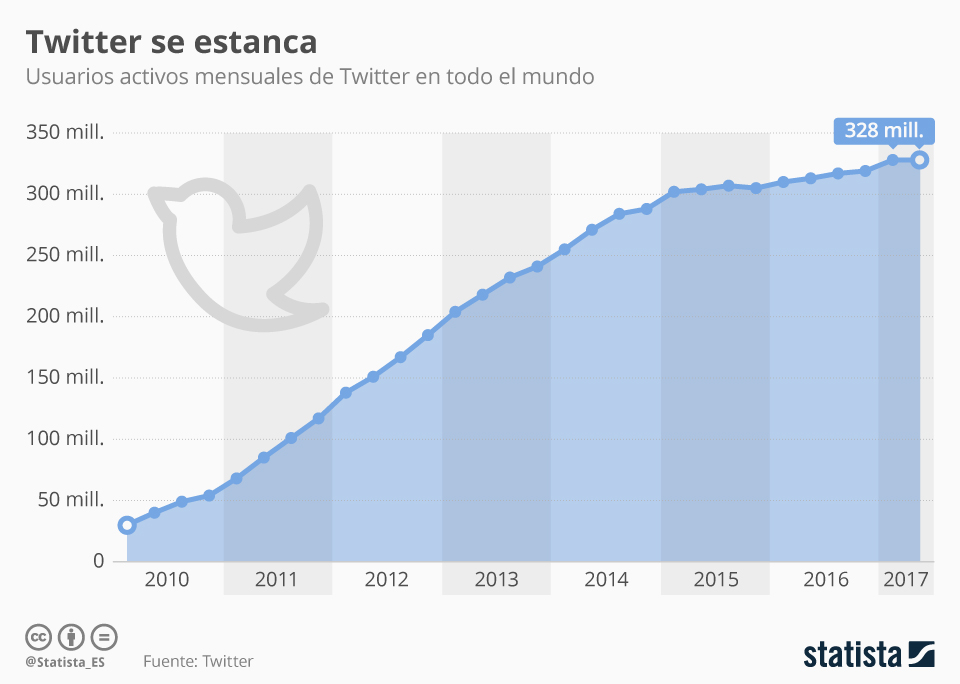
\includegraphics[width=0.4\textwidth]{usuarios_de_twitter}
&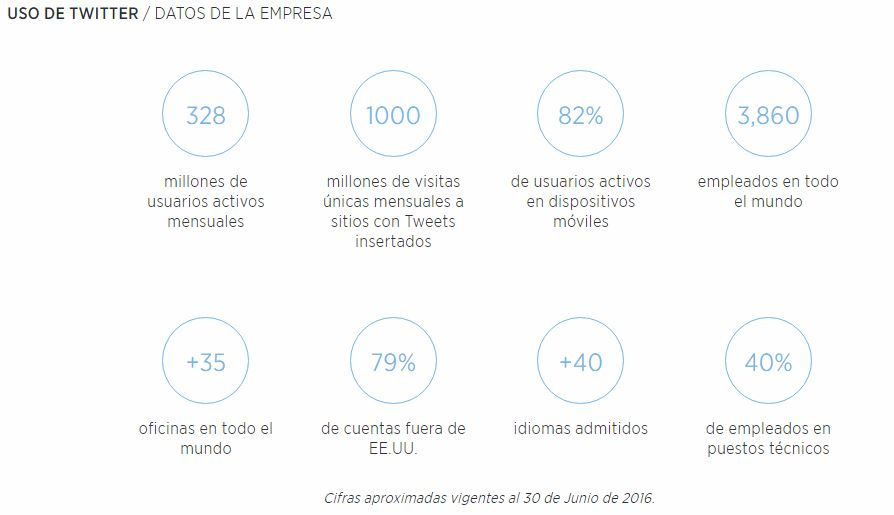
\includegraphics[width=0.4\textwidth]{twitter_uso_y_empresa}
\end{tabular}
\figcaption{Twitter: evolución del número de usuarios (Statista 2017, 
            \url{https://es.statista.com/grafico/10476/el-numero-de-usuarios-de-twitter-se-estanca })
			y datos de la empresa, \url{https://about.twitter.com/es/company }.}
\label{fig:Twitter_uso} }


Esta red da cabida a relaciones diversas, entre usuarios de variada índole. Dado que muchos de los usuarios 
publican información relacionada con su ocupación laboral, es natural esperar que en Twitter 
se formen comunidades de individuos que comparten interés en diferentes aspectos de dicho ámbito.
Nuestro propósito es definir e implementar un proceso que permita agregar información referente a 
esas comunidades a un determinado proceso de selección.

Observemos las dos siguientes ofertas de trabajo aparecidas recientemente (Septiembre 2017) en LinkedIn,
incluyendo los requisitos solicitados a los posibles candidatos:

\myfigure{\begin{tabular}{cc}
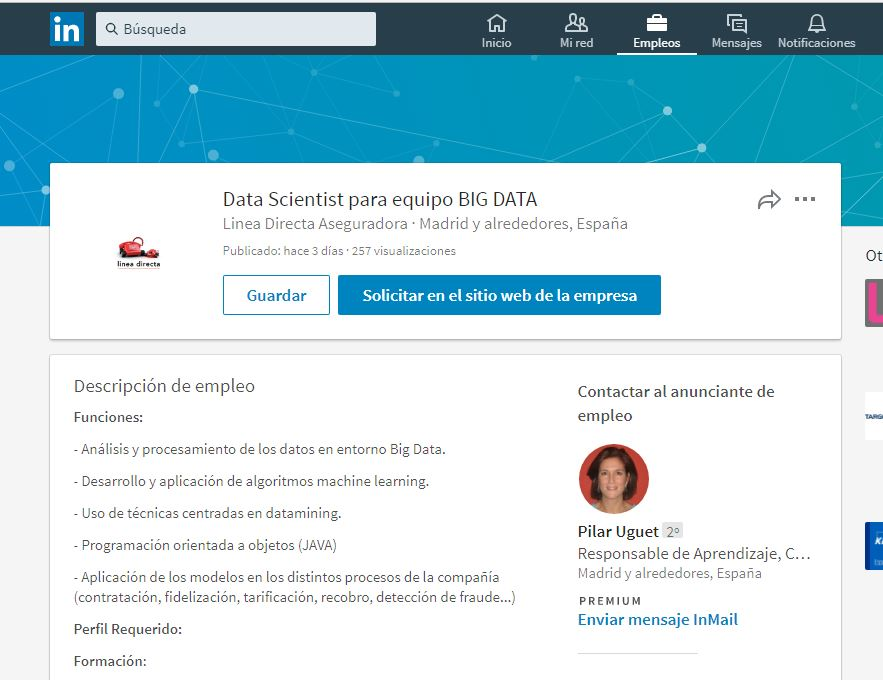
\includegraphics[width=0.4\textwidth]{oferta1_1}
&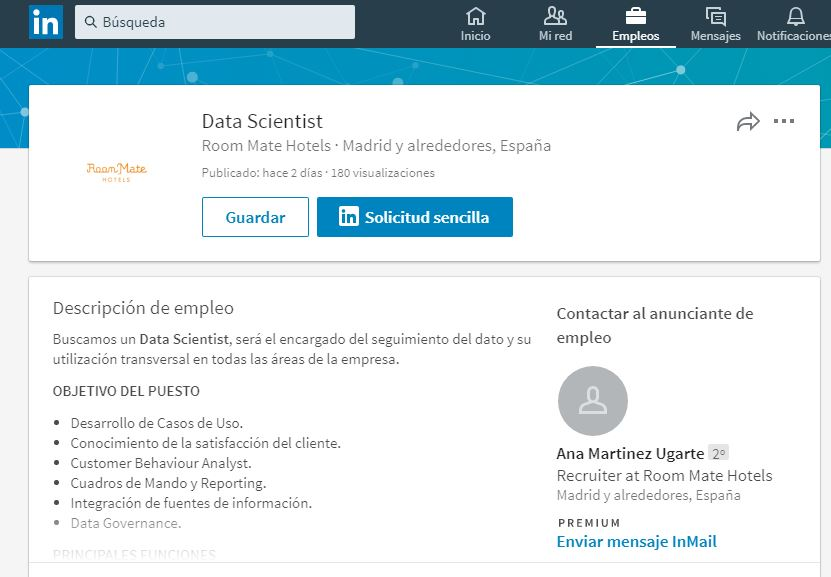
\includegraphics[width=0.4\textwidth]{oferta2_1}
\end{tabular}
\figcaption{Dos ofertas de empleo.}
\label{fig:ofertas_descripcion} }


\myfigure{\begin{tabular}{cc}
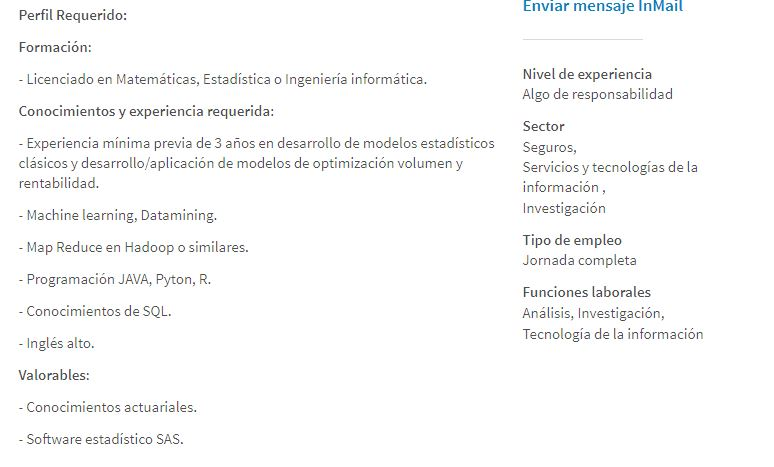
\includegraphics[width=0.4\textwidth]{oferta1_2}
&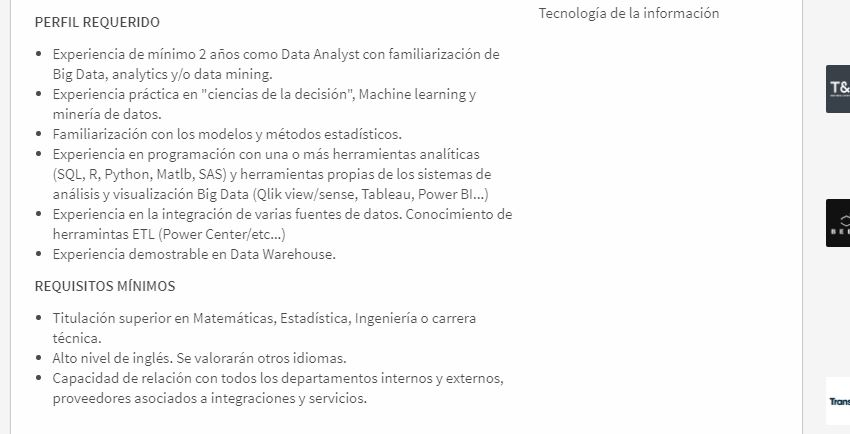
\includegraphics[width=0.4\textwidth]{oferta2_2}
\end{tabular}
\figcaption{Requisitos de las dos ofertas de empleo.}
\label{fig:ofertas_requisitos} }

En ambos casos, entre los requisitos se encuentran conocimientos sobre Python, R,
SQL, machine learning y data mining. Un reclutador probablemente usará esas palabras clave para buscar
los perfiles adecuados para alguno de los dos puestos, y construirá un conjunto de posibles candidatos (el
primer paso en nuestra descripción del proceso de contratación). En esta fase, y gracias a Octopus Data Insights,
nuestro reclutador contará con una ayuda extra. Octopus Data Insights le proporcionará una lista de usuarios
de Twitter que hayan publicado contenido en el que aparezcan esas palabras clave, que complementarán
el resultado que el reclutador haya obtenido por sus propios medios. La información proporcionada
por Octopus Data Insights resultará relevante también más adelante en el proceso,
cuando haya que tomar una decisión entre varios candidatos para determinar cuáles son los más adecuados para el 
puesto: usando la información de Twitter, los usuarios de la lista estarán ordenados según 
diversos criterios de relevancia.

El proceso para producir la información que ayudará al reclutador en el proceso es el siguiente:
\begin{enumerate}
\item Identificar los vocablos que determinan las habilidades que ha de poseer cualquier candidato
para la oferta en cuestión y extraer de Twitter aquellos tuits con contenido relacionado con ellos.
\item Dados esos tuits, construir un conjunto de usuarios, que entendemos como posibles candidatos 
a la oferta.
\item Usar la información publicada por los usuarios para determinar el grado de adecuación a la oferta
(serán más adecuados aquellos que hayan publicado información sobre todos los conocimientos requeridos que 
aquellos que solo hayan publicado sobre alguno de ellos, y más relevantes aquellos más activos, según el
número de tuits publicados sobre cada área).
\item Estudiar la relación entre los usuarios de este conjunto, y determinar los más relevantes en sentido
relativo (en términos de actividad en la red, cuáles son los más ``retuiteados", cuáles los más seguidos, etc.).
\end{enumerate}



\section{Contexto de negocio}
Lo que hay hecho y lo que no.
\section{Objetivos}
Lo que queremos conseguir, qué significa que lo hayamos conseguido.
\section{Hip\'otesis y limitaciones}
Aquí todo lo que asumamos al plantear el proyecto, y hasta dónde puede llegar. Límites del uso de la información
de las redes sociales, límites del proceso en sí (ventana temporal, no detección de todos los candidatos, etc.).

La hipótesis fundamental que estamos haciendo al iniciar este proceso, es que la actividad en Twitter
acerca de un determinado tema (por ejemplo, publicar algo relacionado con Python), supone
que el usuario en cuestión tiene conocimientos sobre dicho tema (en nuestro caso, entenderíamos que ese
usuario posee conocimientos de Python). Esto es cuestionable, por supuesto, pero también ponderable
si tenemos en cuenta que la actividad no sea esporádica. Si un usuario publica sobre un tema
en numerosas ocasiones, la hipótesis de que ese tema no le resulta ajeno, va cobrando fuerza.

Entre las limitaciones de las que adolece el proceso definido para llevar a cabo el proyecto, se encuentran las 
siguientes:
\begin{enumerate}
\item En general, no todos los posibles candidatos tienen por qué usar Twitter, y por tanto habrá muchos que 
queden directamente fuera de nuestro proceso.
\item Los tuits utilizados en el proceso están sujetos a una ventana temporal. Habrá muchos candidatos,
usuarios de Twitter, que no aparezcan en nuestros registros, por no presentar actividad durante ese tiempo.
\item Twitter impone limitaciones en la cantidad de información a la que deja acceder, y por ello, también es
posible que los usuarios pierdad visibilidad en este proceso, 
porque el contenido publicado por ellos no se encuentre entre el proporcionado por la red social durante el proceso
de extracción de datos.
\end{enumerate}


Otra limitación del proceso es que la información que obtenemos de la red es a nivel de usuario de Twitter. 
La dirección de correo o el nombre verdadero de la persona en cuestión, o cualquier dato que pudiera identificarla
no está necesariamente disponible en la aplicación, salvo que el usuario lo haya querido hacer público explícitamente. 
Esta información, y la forma en que se utilice, es clave para la usabilidad del resultado del proyecto, en dos aspectos principales:
\begin{enumerate}
\item para que el reclutador pueda hacer uso de la información, la persona ha de estar identificada, lo suficientemente
como para abrir un canal de comunicación entre el reclutador y el posible candidato.
\item Desde el punto de vista de la comercialización del resultado del proyecto, el hecho de identificar usuarios en una red
social y usar esa información con fines lucrativos, ha de ser implementado de forma muy cuidadosa. El impacto de la Ley 
Orgánica de Protección de Datos de Carácter Personal (LOPD) es muy relevante en nuestro proyecto, y merece un apartado especial.
Nos ocupamos de ello en la sección \ref{subsection:LOPD}.
\end{enumerate}
En relación al primer punto, evidentemente proporcionar un usuario de Twitter ya es abrir un canal de
comunicación. Sin embargo, solo la información de las publicaciones del usuario no es suficiente para 
incluirlo en un proceso de selección, incluso antes del primer contacto entre reclutador y candidato,
y el primero probablemente  necesitará más información (por ejemplo un CV) para considerar al segundo. 
Una forma de solventarlo sería cruzar la información de Twitter (el nombre de usuario)
con la contenida en otros portales (como LinkedIn,  Facebook, Academia.edu, ResearchGate, Glassdoor, etc.),
ya que a menudo el usuario de Twitter es parte de los datos consignados en los CV. Esta extensión
del proyecto la hemos dejado deliberadamente fuera del planteamiento de este proyecto, aunque sería 
{\em conditio sine qua non} para una implementación comercializable del proyecto.




\subsection{La Ley Orgánica 15/1999, de 13 de diciembre, de Protección de Datos
de Carácter Personal}
\label{subsection:LOPD}

La Agencia Española de Protección de Datos, AEDP, define un dato de carácter personal del siguiente modo:

\myfigure{
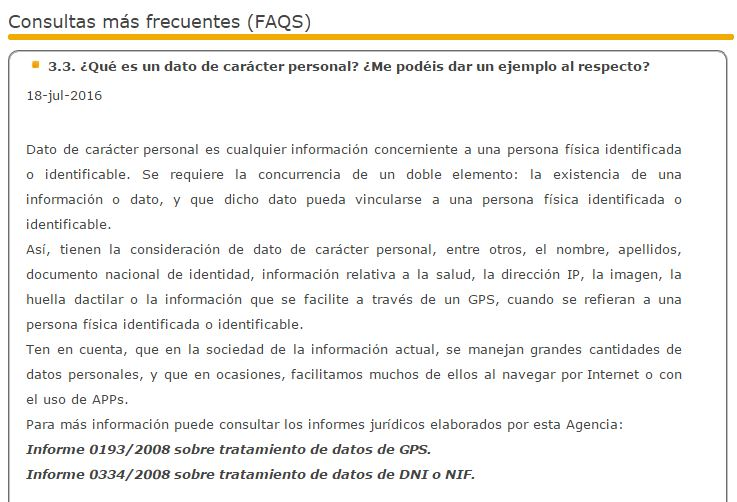
\includegraphics[width=0.6\textwidth]{dato_personal}
\figcaption{AEDP preguntas frecuentes,
           \url{https://sedeagpd.gob.es/sede-electronica-web/vistas/infoSede/detallePreguntaFAQ.jsf;jsessionid=147951A8A98D206E87F2655B9E96E7EB?idPregunta=FAQ%2F00025%
		   }} 
\label{fig:dato_personal} }

El perfil en Twitter de un usuario se puede considerar por tanto un dato de carácter personal, en tanto en cuanto
permitiría localizar e identificar al usuario, tal vez a través de cruces de la información en Twitter con
información adicional (por ejemplo, lo que comentábamos a propósito de encontrar el CV del usuario usando que
frecuentemente, el usuario de Twitter es parte de la información contenida en el mismo, y el CV está disponible en otros 
portales). Sin embargo, en la política de privacidad de Twitter (\url{https://twitter.com/es/privacy })
se establece que
\begin{center}
\noindent\begin{minipage}{0.9\linewidth}%{0.9\columnwidth}
\centering%
{\em ''Al utilizar cualquiera de nuestros Servicios, usted da su consentimiento para la recopilación, 
 la transferencia, la manipulación, el almacenamiento, la revelación y otros usos de su información 
 según lo descrito en esta Política de Privacidad. Esto incluye cualquier información que elija proporcionar que 
 se considere sensible según la legislación vigente."}
\end{minipage}
\end{center}
Y también, en relación a la información del perfil o publicaciones:
\begin{center}
\noindent\begin{minipage}{0.9\linewidth}%{0.9\columnwidth}
\centering%
{\em ''{\bf Información básica de la cuenta}: si opta por crear una cuenta de Twitter, debe promocionar cierta información personal, 
como su nombre, nombre de usuario, contraseña, dirección de correo electrónico o número de teléfono. 
En Twitter, su nombre y nombre de usuario siempre se hacen públicos, incluso en su página de perfil y en los resultados de búsqueda, 
y puede utilizar su nombre real o un seudónimo."

''{\bf Tuits, gente que sigue, listas, perfil y otra información pública}: Twitter está principalmente diseñado para ayudarle a 
compartir información con el mundo. La mayoría de la información que usted nos facilita a través de Twitter es información 
que nos está pidiendo que hagamos pública. Puede facilitarnos información de perfil para hacerla pública en Twitter, como por 
ejemplo, una breve biografía, su ubicación, su sitio web, fecha de nacimiento, o una fotografía. Además, su información pública 
incluye los mensajes que tuitea; los metadatos facilitados con los tuits, tales como cuándo ha tuiteado y la aplicación cliente 
que utilizó para tuitear; información sobre su cuenta, como el momento de su creación, el idioma, el país y la zona horaria; y las 
listas que crea, las personas a las que sigue, los tuits que retuitea o marca como Me gusta, y las emisiones de Periscope en las que 
hace clic o con las que se relaciona de alguna forma (por ejemplo, haciendo comentarios o clic en el icono de corazón) en Twitter. 
Twitter disemina amplia e instantáneamente su información pública a una amplia gama de usuarios, clientes y servicios, incluyendo 
motores de búsqueda, desarrolladores y editores que integran contenido de Twitter en sus servicios y organizaciones, tales como universidades, 
agencias de salud pública y empresas de investigación de mercado que analizan la información en busque de tendencias y conocimiento."}
\end{minipage}
\end{center}
A tenor de estas afirmaciones, la información que nosotros vamos a manejar en la implementación de este proyecto
(nombre de usuario, información del perfil, tuits publicados)
es una información de carácter público. 

En su enunciado, la LOPD establece que
(texto extraído del informe jurídico  2013-0184 de la AEPD
\url{http://www.agpd.es/portalwebAGPD/canaldocumentacion/informes_juridicos/otras_cuestiones/common/pdfs/2013-0184_Red-social-y-creaci-oo-n-de-perfiles-de-empleados..pdf%
})
\begin{center}
\noindent\begin{minipage}{0.9\linewidth}%{0.9\columnwidth}
\centering%
{\em Establece a este
respecto la Ley Orgánica 15/1999 en su artículo 2 que ''El régimen de
protección de los datos de carácter personal que se establece en la
presente Ley Orgánica no será de aplicación: a) A los ficheros
mantenidos por personas físicas en el ejercicio de actividades
exclusivamente personales o domésticas."
}
\end{minipage}
\end{center}

Y define las actividades personales a continuación:

\begin{center}
\noindent\begin{minipage}{0.9\linewidth}%{0.9\columnwidth}
\centering%
{\em
En cuanto a la determinación de que se entiende por actividades
personales o domésticas dispone el Reglamento de desarrollo de la LOPD en
su artículo 4 que ''Sólo se considerarán relacionados con actividades
personales o domésticas los tratamientos relativos a las actividades que se
inscriben en el marco de la vida privada o familiar de los particulares."
Esta es también la interpretación del término ''personal" contenida en la
Sentencia de la Audiencia Nacional de 15 de junio de 2006 al señalar que ''(…)
Será personal cuando los datos tratados afecten a la esfera más íntima de la
persona, a sus relaciones familiares y de amistad y que la finalidad del
tratamiento no sea otra que surtir efectos en esos ámbitos.

También dará lugar a la aplicación de la Ley Orgánica 15/1999, por
superar el ámbito de la vida privada o familiar de los particulares la publicación
de datos de terceros en la red cuando no existan limitaciones de acceso a su
perfil, en cuanto que dicha publicación constituye una cesión de datos, definida
en el artículo 3 j) de la LOPD como “Toda revelación de datos realizada a una
persona distinta del interesado”, ya que en estos supuestos, como señalaba la
sentencia la Sentencia de 6 de noviembre de 2003 (caso Bodil Lindqvist) del
Tribunal de Justicia de las Comunidades Europeas, no se inscribe en el marco
de la vida privada o familiar de los particulares “un tratamiento de datos
personales consistente en la difusión de dichos datos por Internet de modo que
resulten accesibles a un grupo indeterminado de personas.”}
\end{minipage}
\end{center}




Refiriéndose incluso a datos de carácter público que aparecen en los datos,
la interpretación de la LOPD respecto al uso de los mismos por terceros, especialmente
en el caso en el que la finalidad de dicho uso sea comercial, es que el único medio
para legitimar el uso es el consentimiento explícito de la persona cuyos datos van 
a utilizarse. Este consentimiento ha de cumplir unas determinadas condiciones
(de nuevo extraemos del informe jurídico  2013-0184 de la AEPD)
\begin{center}
\noindent\begin{minipage}{0.9\linewidth}%{0.9\columnwidth}
\centering%
{\em 
El tratamiento de datos de carácter personal debe encontrarse fundado
en alguna de las causas legitimadoras previstas en el artículo 6 de la Ley
Orgánica 15/1999, disponiendo a este respecto su número primero que ''El
tratamiento de los datos de carácter personal requerirá el consentimiento
inequívoco del afectado, salvo que la ley disponga otra cosa."

(\dots)

Dicho
consentimiento debe reunir las características señaladas en el
artículo 3.h de la misma Ley que lo define como ''manifestación de
voluntad, libre, inequívoca, específica e informada, mediante la que el
interesado consienta el tratamiento de datos personales que le
conciernen".

Esta Agencia ha venido describiendo en sus informes dichas
características de manera que se entiende por consentimiento libre aquel que
ha sido obtenido sin la intervención de vicio alguno del consentimiento en los
términos regulados por el Código Civil.
}
\end{minipage}
\end{center}


\myfigure{
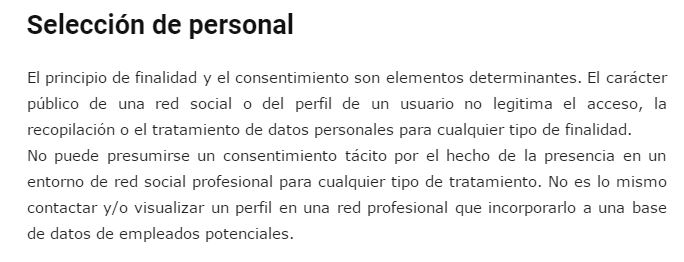
\includegraphics[width=0.6\textwidth]{LOPD1}
\figcaption{Ayuda Ley de Protección de Datos, 
           \url{https://ayudaleyprotecciondatos.es/2010/09/16/redes-sociales-empresas-y-proteccion-de-datos/ }}
\label{fig:LOPD1} }


Como consecuencia de toda esta información, entendemos lo siguiente:
\begin{itemize}
\item que los datos del perfil de los usuarios de Twitter, así como sus publicaciones en dicha red,
tienen carácter público.
\item Que el carácter público de dichos datos no es óbice para poder manipularlos y distribuirlos
a terceros, en ninguna actividad que no se circunscriba al ámbito personal o familiar.
\item La elaboración de un proyecto de fin de máster no tiene por qué entenderse como una 
actividad del ámbito personal o familiar, con lo cual no estaría en disposición de difundir esa información
a terceros, salvo en las condiciones previstas en la LOPD.
\item Cualquier versión comercializable de este proyecto debería contar con los mecanismos
adecuados para obtener el consentimiento explícito de los usuarios para el uso de sus perfiles, 
y posible inclusión en un proceso de selección de personal. Esta fase quedará fuera del plan de elaboración
del proyecto.
\end{itemize}
Para eliminar el riesgo relativo a protección de datos en la elaboración del proyecto, 
pero sin alterar su esencia, proponemos publicar los resultados enmascarando los nombres de usuario 
de aquellos que aparezcan en nuestra base de datos.

